%\usepackage{array}
%\usepackage{color}
%\usepackage[table]{xcolor}
%\usepackage{graphics}
%\usepackage{graphicx}
%\usepackage{tabularx}
%\usepackage{booktabs}
%\usepackage{multirow}
%\usepackage{multicol}
%\usepackage{adjustbox} % for \adjincludegraphics
%\usepackage{etoolbox}
%\usepackage[absolute,overlay]{textpos}
%\usepackage{calc}
%\usepackage{fancybox}
%\usepackage{ctable}
%\usepackage{changepage}


\definecolor{hughesblue}{rgb}{.9,.9,1} 





\renewcommand\lstlistingname{R}% Change language of section name

\lstset{ % General setup for the package
	language=R,
	keepspaces=true, % keeps spaces in text
	basicstyle=\small\sffamily,
	numbers=left,
 	numberstyle=\tiny,
 	frame=tb,
	tabsize=4,
	columns=fixed,
	showstringspaces=false,
	showtabs=false,
	keepspaces,
	commentstyle=\color{red},
	keywordstyle=\color{blue}
}


% Printing the Handout
% \usepackage{pgfpages}
% \pgfpagelayout{resize}[a4paper,border shrink=5mm,landscape]
% This says resize all pages to landscape A4 pages, no what their original size was, but shrink the pages by 5mm, so that there is a bit of a border around everything. \pgfpagelayout{2 on 1}[a4paper,border shrink=5mm]

% \usepackage{multimedia}
% A stand-alone package that implements several commands for including external animation and sound
%\setbeamertemplate{blocks}[rounded][shadow=true]

\newcommand{\backupbegin}{%
   \newcounter{framenumberappendix}
   \setcounter{framenumberappendix}{\value{framenumber}}
}%
\newcommand{\backupend}{%
   \addtocounter{framenumberappendix}{-\value{framenumber}}
   \addtocounter{framenumber}{\value{framenumberappendix}}
}%


\title{Comunidades Terapêuticas}
\subtitle{}
\date{October 2, 2015}
\author{Daniel Marcelino}
\institute{Instituto de Pesquisa Econômica Aplicada}

\usepackage{Sweave}
\begin{document}
\Sconcordance{concordance:CT-2016.tex:CT-2016.Rnw:%
1 15 1 1 0 210 1}


\maketitle
\AtBeginSection{\frame{\sectionpage}}

\begin{frame}{Overview}
\tableofcontents
\end{frame}

\section{Introdução}
\begin{frame}{Conceito em construção}
\input{sections/introducao.tex}
\end{frame}

\section{Conceito}
\begin{frame}{Conceito em construção}
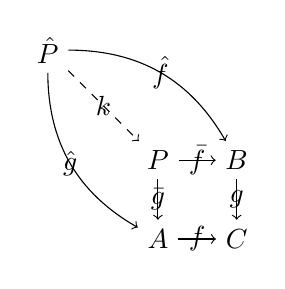
\begin{tikzpicture}
\node (P) {$P$};
\node (B) [right of=P] {$B$};
\node (A) [below of=P] {$A$};
\node (C) [below of=B] {$C$};
\node (P1) [node distance=1.4cm, left of=P, above of=P] {$\hat{P}$};
\draw[->] (P) to node {$\bar{f}$} (B);
\draw[->] (P) to node [swap] {$\bar{g}$} (A);
\draw[->] (A) to node [swap] {$f$} (C);
\draw[->] (B) to node {$g$} (C);
\draw[->, bend right] (P1) to node [swap] {$\hat{g}$} (A);
\draw[->, bend left] (P1) to node {$\hat{f}$} (B);
\draw[->, dashed] (P1) to node {$k$} (P);
\end{tikzpicture}



\end{frame}

% The Problem of (Weak) Priors
\section{The Problem of (Weak) Priors}

\begin{frame}
\begin{exampleblock}{Example}

\end{exampleblock}

\end{frame}

\begin{frame}
\begin{block}{Block}

\end{block}

\end{frame}


\appendix

\backupbegin

\begin{frame}[fragile]

\begin{lstlisting}
require(SciencesPo)
crosstable(data, var1, var2, var3, row=TRUE)
\end{lstlisting}

\end{frame}

\backupend

\end{document}

